\documentclass[1p]{elsarticle_modified}
%\bibliographystyle{elsarticle-num}

%\usepackage[colorlinks]{hyperref}
%\usepackage{abbrmath_seonhwa} %\Abb, \Ascr, \Acal ,\Abf, \Afrak
\usepackage{amsfonts}
\usepackage{amssymb}
\usepackage{amsmath}
\usepackage{amsthm}
\usepackage{scalefnt}
\usepackage{amsbsy}
\usepackage{kotex}
\usepackage{caption}
\usepackage{subfig}
\usepackage{color}
\usepackage{graphicx}
\usepackage{xcolor} %% white, black, red, green, blue, cyan, magenta, yellow
\usepackage{float}
\usepackage{setspace}
\usepackage{hyperref}

\usepackage{tikz}
\usetikzlibrary{arrows}

\usepackage{multirow}
\usepackage{array} % fixed length table
\usepackage{hhline}

%%%%%%%%%%%%%%%%%%%%%
\makeatletter
\renewcommand*\env@matrix[1][\arraystretch]{%
	\edef\arraystretch{#1}%
	\hskip -\arraycolsep
	\let\@ifnextchar\new@ifnextchar
	\array{*\c@MaxMatrixCols c}}
\makeatother %https://tex.stackexchange.com/questions/14071/how-can-i-increase-the-line-spacing-in-a-matrix
%%%%%%%%%%%%%%%

\usepackage[normalem]{ulem}

\newcommand{\msout}[1]{\ifmmode\text{\sout{\ensuremath{#1}}}\else\sout{#1}\fi}
%SOURCE: \msout is \stkout macro in https://tex.stackexchange.com/questions/20609/strikeout-in-math-mode

\newcommand{\cancel}[1]{
	\ifmmode
	{\color{red}\msout{#1}}
	\else
	{\color{red}\sout{#1}}
	\fi
}

\newcommand{\add}[1]{
	{\color{blue}\uwave{#1}}
}

\newcommand{\replace}[2]{
	\ifmmode
	{\color{red}\msout{#1}}{\color{blue}\uwave{#2}}
	\else
	{\color{red}\sout{#1}}{\color{blue}\uwave{#2}}
	\fi
}

\newcommand{\Sol}{\mathcal{S}} %segment
\newcommand{\D}{D} %diagram
\newcommand{\A}{\mathcal{A}} %arc


%%%%%%%%%%%%%%%%%%%%%%%%%%%%%5 test

\def\sl{\operatorname{\textup{SL}}(2,\Cbb)}
\def\psl{\operatorname{\textup{PSL}}(2,\Cbb)}
\def\quan{\mkern 1mu \triangleright \mkern 1mu}

\theoremstyle{definition}
\newtheorem{thm}{Theorem}[section]
\newtheorem{prop}[thm]{Proposition}
\newtheorem{lem}[thm]{Lemma}
\newtheorem{ques}[thm]{Question}
\newtheorem{cor}[thm]{Corollary}
\newtheorem{defn}[thm]{Definition}
\newtheorem{exam}[thm]{Example}
\newtheorem{rmk}[thm]{Remark}
\newtheorem{alg}[thm]{Algorithm}

\newcommand{\I}{\sqrt{-1}}
\begin{document}

%\begin{frontmatter}
%
%\title{Boundary parabolic representations of knots up to 8 crossings}
%
%%% Group authors per affiliation:
%\author{Yunhi Cho} 
%\address{Department of Mathematics, University of Seoul, Seoul, Korea}
%\ead{yhcho@uos.ac.kr}
%
%
%\author{Seonhwa Kim} %\fnref{s_kim}}
%\address{Center for Geometry and Physics, Institute for Basic Science, Pohang, 37673, Korea}
%\ead{ryeona17@ibs.re.kr}
%
%\author{Hyuk Kim}
%\address{Department of Mathematical Sciences, Seoul National University, Seoul 08826, Korea}
%\ead{hyukkim@snu.ac.kr}
%
%\author{Seokbeom Yoon}
%\address{Department of Mathematical Sciences, Seoul National University, Seoul, 08826,  Korea}
%\ead{sbyoon15@snu.ac.kr}
%
%\begin{abstract}
%We find all boundary parabolic representation of knots up to 8 crossings.
%
%\end{abstract}
%\begin{keyword}
%    \MSC[2010] 57M25 
%\end{keyword}
%
%\end{frontmatter}

%\linenumbers
%\tableofcontents
%
\newcommand\colored[1]{\textcolor{white}{\rule[-0.35ex]{0.8em}{1.4ex}}\kern-0.8em\color{red} #1}%
%\newcommand\colored[1]{\textcolor{white}{ #1}\kern-2.17ex	\textcolor{white}{ #1}\kern-1.81ex	\textcolor{white}{ #1}\kern-2.15ex\color{red}#1	}

{\Large $\underline{12a_{0106}~(K12a_{0106})}$}

\setlength{\tabcolsep}{10pt}
\renewcommand{\arraystretch}{1.6}
\vspace{1cm}\begin{tabular}{m{100pt}>{\centering\arraybackslash}m{274pt}}
\multirow{5}{120pt}{
	\centering
	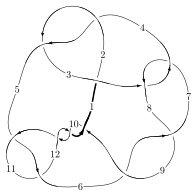
\includegraphics[width=112pt]{../../../GIT/diagram.site/Diagrams/png/907_12a_0106.png}\\
\ \ \ A knot diagram\footnotemark}&
\allowdisplaybreaks
\textbf{Linearized knot diagam} \\
\cline{2-2}
 &
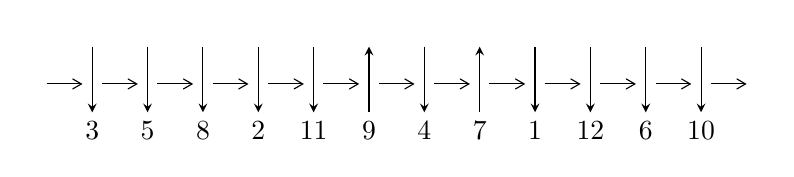
\begin{tikzpicture}[x=20pt, y=17pt]
	% nodes
	\node (C0) at (0, 0) {};
	\node (C1) at (1, 0) {};
	\node (C1U) at (1, +1) {};
	\node (C1D) at (1, -1) {3};

	\node (C2) at (2, 0) {};
	\node (C2U) at (2, +1) {};
	\node (C2D) at (2, -1) {5};

	\node (C3) at (3, 0) {};
	\node (C3U) at (3, +1) {};
	\node (C3D) at (3, -1) {8};

	\node (C4) at (4, 0) {};
	\node (C4U) at (4, +1) {};
	\node (C4D) at (4, -1) {2};

	\node (C5) at (5, 0) {};
	\node (C5U) at (5, +1) {};
	\node (C5D) at (5, -1) {11};

	\node (C6) at (6, 0) {};
	\node (C6U) at (6, +1) {};
	\node (C6D) at (6, -1) {9};

	\node (C7) at (7, 0) {};
	\node (C7U) at (7, +1) {};
	\node (C7D) at (7, -1) {4};

	\node (C8) at (8, 0) {};
	\node (C8U) at (8, +1) {};
	\node (C8D) at (8, -1) {7};

	\node (C9) at (9, 0) {};
	\node (C9U) at (9, +1) {};
	\node (C9D) at (9, -1) {1};

	\node (C10) at (10, 0) {};
	\node (C10U) at (10, +1) {};
	\node (C10D) at (10, -1) {12};

	\node (C11) at (11, 0) {};
	\node (C11U) at (11, +1) {};
	\node (C11D) at (11, -1) {6};

	\node (C12) at (12, 0) {};
	\node (C12U) at (12, +1) {};
	\node (C12D) at (12, -1) {10};
	\node (C13) at (13, 0) {};

	% arrows
	\draw[->,>={angle 60}]
	(C0) edge (C1) (C1) edge (C2) (C2) edge (C3) (C3) edge (C4) (C4) edge (C5) (C5) edge (C6) (C6) edge (C7) (C7) edge (C8) (C8) edge (C9) (C9) edge (C10) (C10) edge (C11) (C11) edge (C12) (C12) edge (C13) ;	\draw[->,>=stealth]
	(C1U) edge (C1D) (C2U) edge (C2D) (C3U) edge (C3D) (C4U) edge (C4D) (C5U) edge (C5D) (C6D) edge (C6U) (C7U) edge (C7D) (C8D) edge (C8U) (C9U) edge (C9D) (C10U) edge (C10D) (C11U) edge (C11D) (C12U) edge (C12D) ;
	\end{tikzpicture} \\
\hhline{~~} \\& 
\textbf{Solving Sequence} \\ \cline{2-2} 
 &
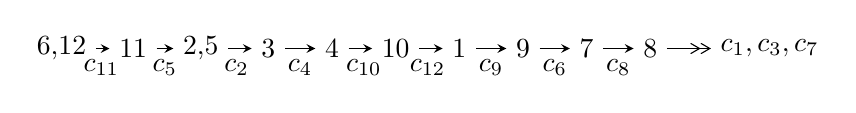
\begin{tikzpicture}[x=23pt, y=7pt]
	% node
	\node (A0) at (-1/8, 0) {6,12};
	\node (A1) at (1, 0) {11};
	\node (A2) at (33/16, 0) {2,5};
	\node (A3) at (25/8, 0) {3};
	\node (A4) at (33/8, 0) {4};
	\node (A5) at (41/8, 0) {10};
	\node (A6) at (49/8, 0) {1};
	\node (A7) at (57/8, 0) {9};
	\node (A8) at (65/8, 0) {7};
	\node (A9) at (73/8, 0) {8};
	\node (C1) at (1/2, -1) {$c_{11}$};
	\node (C2) at (3/2, -1) {$c_{5}$};
	\node (C3) at (21/8, -1) {$c_{2}$};
	\node (C4) at (29/8, -1) {$c_{4}$};
	\node (C5) at (37/8, -1) {$c_{10}$};
	\node (C6) at (45/8, -1) {$c_{12}$};
	\node (C7) at (53/8, -1) {$c_{9}$};
	\node (C8) at (61/8, -1) {$c_{6}$};
	\node (C9) at (69/8, -1) {$c_{8}$};
	\node (A10) at (11, 0) {$c_{1},c_{3},c_{7}$};

	% edge
	\draw[->,>=stealth]	
	(A0) edge (A1) (A1) edge (A2) (A2) edge (A3) (A3) edge (A4) (A4) edge (A5) (A5) edge (A6) (A6) edge (A7) (A7) edge (A8) (A8) edge (A9) ;
	\draw[->>,>={angle 60}]	
	(A9) edge (A10);
\end{tikzpicture} \\ 

\end{tabular} \\

\footnotetext{
The image of knot diagram is generated by the software ``\textbf{Draw programme}" developed by Andrew Bartholomew(\url{http://www.layer8.co.uk/maths/draw/index.htm\#Running-draw}), where we modified some parts for our purpose(\url{https://github.com/CATsTAILs/LinksPainter}).
}\phantom \\ \newline 
\centering \textbf{Ideals for irreducible components\footnotemark of $X_{\text{par}}$} 
 
\begin{align*}
I^u_{1}&=\langle 
u^{73}+u^{72}+\cdots-2 u^2+b,\;- u^{43}+6 u^{41}+\cdots+a-2,\;u^{75}+2 u^{74}+\cdots+2 u+1\rangle \\
I^u_{2}&=\langle 
-2 u^2+b+2 u+1,\;a+u,\;u^3- u^2+1\rangle \\
\\
\end{align*}
\raggedright * 2 irreducible components of $\dim_{\mathbb{C}}=0$, with total 78 representations.\\
\footnotetext{All coefficients of polynomials are rational numbers. But the coefficients are sometimes approximated in decimal forms when there is not enough margin.}
\newpage
\renewcommand{\arraystretch}{1}
\centering \section*{I. $I^u_{1}= \langle u^{73}+u^{72}+\cdots-2 u^2+b,\;- u^{43}+6 u^{41}+\cdots+a-2,\;u^{75}+2 u^{74}+\cdots+2 u+1 \rangle$}
\flushleft \textbf{(i) Arc colorings}\\
\begin{tabular}{m{7pt} m{180pt} m{7pt} m{180pt} }
\flushright $a_{6}=$&$\begin{pmatrix}0\\u\end{pmatrix}$ \\
\flushright $a_{12}=$&$\begin{pmatrix}1\\0\end{pmatrix}$ \\
\flushright $a_{11}=$&$\begin{pmatrix}1\\- u^2\end{pmatrix}$ \\
\flushright $a_{2}=$&$\begin{pmatrix}u^{43}-6 u^{41}+\cdots-2 u+2\\- u^{73}- u^{72}+\cdots-3 u^3+2 u^2\end{pmatrix}$ \\
\flushright $a_{5}=$&$\begin{pmatrix}u\\- u^3+u\end{pmatrix}$ \\
\flushright $a_{3}=$&$\begin{pmatrix}- u^{74}- u^{73}+\cdots-4 u+1\\- u^{74}- u^{73}+\cdots+3 u^2- u\end{pmatrix}$ \\
\flushright $a_{4}=$&$\begin{pmatrix}- u^{74}- u^{73}+\cdots+2 u-2\\- u^{74}+u^{73}+\cdots+6 u^3-3 u^2\end{pmatrix}$ \\
\flushright $a_{10}=$&$\begin{pmatrix}- u^2+1\\- u^2\end{pmatrix}$ \\
\flushright $a_{1}=$&$\begin{pmatrix}u^4- u^2+1\\u^4\end{pmatrix}$ \\
\flushright $a_{9}=$&$\begin{pmatrix}- u^6+u^4-2 u^2+1\\- u^6- u^2\end{pmatrix}$ \\
\flushright $a_{7}=$&$\begin{pmatrix}u^{13}-2 u^{11}+5 u^9-6 u^7+6 u^5-4 u^3+u\\u^{13}- u^{11}+3 u^9-2 u^7+2 u^5- u^3+u\end{pmatrix}$ \\
\flushright $a_{8}=$&$\begin{pmatrix}- u^{20}+3 u^{18}+\cdots- u^2+1\\- u^{20}+2 u^{18}-6 u^{16}+8 u^{14}-11 u^{12}+10 u^{10}-8 u^8+4 u^6-3 u^4\end{pmatrix}$\\&\end{tabular}
\flushleft \textbf{(ii) Obstruction class $= -1$}\\~\\
\flushleft \textbf{(iii) Cusp Shapes $= 3 u^{74}+2 u^{73}+\cdots+9 u-11$}\\~\\
\newpage\renewcommand{\arraystretch}{1}
\flushleft \textbf{(iv) u-Polynomials at the component}\newline \\
\begin{tabular}{m{50pt}|m{274pt}}
Crossings & \hspace{64pt}u-Polynomials at each crossing \\
\hline $$\begin{aligned}c_{1}\end{aligned}$$&$\begin{aligned}
&u^{75}+42 u^{74}+\cdots+39 u+1
\end{aligned}$\\
\hline $$\begin{aligned}c_{2},c_{4}\end{aligned}$$&$\begin{aligned}
&u^{75}-4 u^{74}+\cdots- u+1
\end{aligned}$\\
\hline $$\begin{aligned}c_{3},c_{7}\end{aligned}$$&$\begin{aligned}
&u^{75}+u^{74}+\cdots+20 u+8
\end{aligned}$\\
\hline $$\begin{aligned}c_{5},c_{11}\end{aligned}$$&$\begin{aligned}
&u^{75}+2 u^{74}+\cdots+2 u+1
\end{aligned}$\\
\hline $$\begin{aligned}c_{6},c_{8}\end{aligned}$$&$\begin{aligned}
&u^{75}-21 u^{74}+\cdots-752 u+64
\end{aligned}$\\
\hline $$\begin{aligned}c_{9},c_{10},c_{12}\end{aligned}$$&$\begin{aligned}
&u^{75}+20 u^{74}+\cdots+14 u+1
\end{aligned}$\\
\hline
\end{tabular}\\~\\
\newpage\renewcommand{\arraystretch}{1}
\flushleft \textbf{(v) Riley Polynomials at the component}\newline \\
\begin{tabular}{m{50pt}|m{274pt}}
Crossings & \hspace{64pt}Riley Polynomials at each crossing \\
\hline $$\begin{aligned}c_{1}\end{aligned}$$&$\begin{aligned}
&y^{75}-14 y^{74}+\cdots+943 y-1
\end{aligned}$\\
\hline $$\begin{aligned}c_{2},c_{4}\end{aligned}$$&$\begin{aligned}
&y^{75}-42 y^{74}+\cdots+39 y-1
\end{aligned}$\\
\hline $$\begin{aligned}c_{3},c_{7}\end{aligned}$$&$\begin{aligned}
&y^{75}+21 y^{74}+\cdots-752 y-64
\end{aligned}$\\
\hline $$\begin{aligned}c_{5},c_{11}\end{aligned}$$&$\begin{aligned}
&y^{75}-20 y^{74}+\cdots+14 y-1
\end{aligned}$\\
\hline $$\begin{aligned}c_{6},c_{8}\end{aligned}$$&$\begin{aligned}
&y^{75}+61 y^{74}+\cdots+232704 y-4096
\end{aligned}$\\
\hline $$\begin{aligned}c_{9},c_{10},c_{12}\end{aligned}$$&$\begin{aligned}
&y^{75}+72 y^{74}+\cdots-10 y-1
\end{aligned}$\\
\hline
\end{tabular}\\~\\
\newpage\flushleft \textbf{(vi) Complex Volumes and Cusp Shapes}
$$\begin{array}{c|c|c}  
\text{Solutions to }I^u_{1}& \I (\text{vol} + \sqrt{-1}CS) & \text{Cusp shape}\\
 \hline 
\begin{aligned}
u &= \phantom{-}0.887145 + 0.421919 I \\
a &= -1.304670 + 0.309765 I \\
b &= -1.36625 + 1.06588 I\end{aligned}
 & \phantom{-}0.04333 - 6.34447 I & -7.93297 + 10.47635 I \\ \hline\begin{aligned}
u &= \phantom{-}0.887145 - 0.421919 I \\
a &= -1.304670 - 0.309765 I \\
b &= -1.36625 - 1.06588 I\end{aligned}
 & \phantom{-}0.04333 + 6.34447 I & -7.93297 - 10.47635 I \\ \hline\begin{aligned}
u &= -0.990634 + 0.243871 I \\
a &= \phantom{-}0.370425 - 0.564934 I \\
b &= \phantom{-}0.509716 - 0.608237 I\end{aligned}
 & -4.44660 + 0.09147 I & -11.59766 + 0. I\phantom{ +0.000000I} \\ \hline\begin{aligned}
u &= -0.990634 - 0.243871 I \\
a &= \phantom{-}0.370425 + 0.564934 I \\
b &= \phantom{-}0.509716 + 0.608237 I\end{aligned}
 & -4.44660 - 0.09147 I & -11.59766 + 0. I\phantom{ +0.000000I} \\ \hline\begin{aligned}
u &= \phantom{-}1.000630 + 0.265543 I \\
a &= \phantom{-}2.03967 + 0.36176 I \\
b &= \phantom{-}1.38837 - 1.74230 I\end{aligned}
 & -8.14996 - 1.57539 I & -15.1216 + 0. I\phantom{ +0.000000I} \\ \hline\begin{aligned}
u &= \phantom{-}1.000630 - 0.265543 I \\
a &= \phantom{-}2.03967 - 0.36176 I \\
b &= \phantom{-}1.38837 + 1.74230 I\end{aligned}
 & -8.14996 + 1.57539 I & -15.1216 + 0. I\phantom{ +0.000000I} \\ \hline\begin{aligned}
u &= -1.002040 + 0.280364 I \\
a &= -2.56830 - 0.43571 I \\
b &= -1.18117 - 1.37862 I\end{aligned}
 & -8.06174 + 4.47030 I & \phantom{-0.000000 } 0 \\ \hline\begin{aligned}
u &= -1.002040 - 0.280364 I \\
a &= -2.56830 + 0.43571 I \\
b &= -1.18117 + 1.37862 I\end{aligned}
 & -8.06174 - 4.47030 I & \phantom{-0.000000 } 0 \\ \hline\begin{aligned}
u &= \phantom{-}0.997744 + 0.300446 I \\
a &= \phantom{-}0.162900 + 0.569242 I \\
b &= \phantom{-}0.500726 + 0.752913 I\end{aligned}
 & -4.11035 - 5.87109 I & \phantom{-0.000000 } 0 \\ \hline\begin{aligned}
u &= \phantom{-}0.997744 - 0.300446 I \\
a &= \phantom{-}0.162900 - 0.569242 I \\
b &= \phantom{-}0.500726 - 0.752913 I\end{aligned}
 & -4.11035 + 5.87109 I & \phantom{-0.000000 } 0\\
 \hline 
 \end{array}$$\newpage$$\begin{array}{c|c|c}  
\text{Solutions to }I^u_{1}& \I (\text{vol} + \sqrt{-1}CS) & \text{Cusp shape}\\
 \hline 
\begin{aligned}
u &= -1.023860 + 0.232154 I \\
a &= \phantom{-}2.01282 - 0.17234 I \\
b &= \phantom{-}1.11389 + 1.64325 I\end{aligned}
 & -7.89110 - 4.43076 I & \phantom{-0.000000 } 0 \\ \hline\begin{aligned}
u &= -1.023860 - 0.232154 I \\
a &= \phantom{-}2.01282 + 0.17234 I \\
b &= \phantom{-}1.11389 - 1.64325 I\end{aligned}
 & -7.89110 + 4.43076 I & \phantom{-0.000000 } 0 \\ \hline\begin{aligned}
u &= -0.930948 + 0.071026 I \\
a &= \phantom{-}1.266100 + 0.027107 I \\
b &= \phantom{-}1.047670 + 0.599871 I\end{aligned}
 & -1.97213 - 1.46805 I & -10.98188 + 4.43556 I \\ \hline\begin{aligned}
u &= -0.930948 - 0.071026 I \\
a &= \phantom{-}1.266100 - 0.027107 I \\
b &= \phantom{-}1.047670 - 0.599871 I\end{aligned}
 & -1.97213 + 1.46805 I & -10.98188 - 4.43556 I \\ \hline\begin{aligned}
u &= \phantom{-}1.023180 + 0.307631 I \\
a &= -2.48345 + 0.20439 I \\
b &= -1.21466 + 1.45040 I\end{aligned}
 & -7.44212 - 10.73660 I & \phantom{-0.000000 } 0 \\ \hline\begin{aligned}
u &= \phantom{-}1.023180 - 0.307631 I \\
a &= -2.48345 - 0.20439 I \\
b &= -1.21466 - 1.45040 I\end{aligned}
 & -7.44212 + 10.73660 I & \phantom{-0.000000 } 0 \\ \hline\begin{aligned}
u &= \phantom{-}0.745430 + 0.809040 I \\
a &= -0.366987 - 1.071930 I \\
b &= -2.70214 - 0.22546 I\end{aligned}
 & -1.06539 - 5.24431 I & \phantom{-0.000000 } 0 \\ \hline\begin{aligned}
u &= \phantom{-}0.745430 - 0.809040 I \\
a &= -0.366987 + 1.071930 I \\
b &= -2.70214 + 0.22546 I\end{aligned}
 & -1.06539 + 5.24431 I & \phantom{-0.000000 } 0 \\ \hline\begin{aligned}
u &= \phantom{-}0.882590 + 0.702538 I \\
a &= -0.829874 - 0.592338 I \\
b &= -1.79400 + 1.05298 I\end{aligned}
 & \phantom{-}2.08360 - 2.69427 I & \phantom{-0.000000 } 0 \\ \hline\begin{aligned}
u &= \phantom{-}0.882590 - 0.702538 I \\
a &= -0.829874 + 0.592338 I \\
b &= -1.79400 - 1.05298 I\end{aligned}
 & \phantom{-}2.08360 + 2.69427 I & \phantom{-0.000000 } 0\\
 \hline 
 \end{array}$$\newpage$$\begin{array}{c|c|c}  
\text{Solutions to }I^u_{1}& \I (\text{vol} + \sqrt{-1}CS) & \text{Cusp shape}\\
 \hline 
\begin{aligned}
u &= \phantom{-}0.743473 + 0.453790 I \\
a &= \phantom{-}0.007570 - 0.366607 I \\
b &= -0.316775 + 0.512887 I\end{aligned}
 & \phantom{-}1.49999 - 2.25964 I & -3.17178 + 5.04191 I \\ \hline\begin{aligned}
u &= \phantom{-}0.743473 - 0.453790 I \\
a &= \phantom{-}0.007570 + 0.366607 I \\
b &= -0.316775 - 0.512887 I\end{aligned}
 & \phantom{-}1.49999 + 2.25964 I & -3.17178 - 5.04191 I \\ \hline\begin{aligned}
u &= \phantom{-}0.795943 + 0.812291 I \\
a &= -0.495301 - 0.730597 I \\
b &= -0.970310 + 0.264145 I\end{aligned}
 & \phantom{-}2.31304 - 1.29591 I & \phantom{-0.000000 } 0 \\ \hline\begin{aligned}
u &= \phantom{-}0.795943 - 0.812291 I \\
a &= -0.495301 + 0.730597 I \\
b &= -0.970310 - 0.264145 I\end{aligned}
 & \phantom{-}2.31304 + 1.29591 I & \phantom{-0.000000 } 0 \\ \hline\begin{aligned}
u &= -0.786206 + 0.833290 I \\
a &= -0.548362 + 1.180140 I \\
b &= -3.10995 - 0.03398 I\end{aligned}
 & -1.046790 - 0.233605 I & \phantom{-0.000000 } 0 \\ \hline\begin{aligned}
u &= -0.786206 - 0.833290 I \\
a &= -0.548362 - 1.180140 I \\
b &= -3.10995 + 0.03398 I\end{aligned}
 & -1.046790 + 0.233605 I & \phantom{-0.000000 } 0 \\ \hline\begin{aligned}
u &= \phantom{-}0.788338 + 0.844997 I \\
a &= -0.39372 + 2.64094 I \\
b &= \phantom{-}3.47934 + 2.39014 I\end{aligned}
 & -0.77118 + 3.07466 I & \phantom{-0.000000 } 0 \\ \hline\begin{aligned}
u &= \phantom{-}0.788338 - 0.844997 I \\
a &= -0.39372 - 2.64094 I \\
b &= \phantom{-}3.47934 - 2.39014 I\end{aligned}
 & -0.77118 - 3.07466 I & \phantom{-0.000000 } 0 \\ \hline\begin{aligned}
u &= -0.795768 + 0.856610 I \\
a &= -0.458519 + 0.581639 I \\
b &= -0.661200 - 0.385202 I\end{aligned}
 & \phantom{-}3.38785 - 4.33505 I & \phantom{-0.000000 } 0 \\ \hline\begin{aligned}
u &= -0.795768 - 0.856610 I \\
a &= -0.458519 - 0.581639 I \\
b &= -0.661200 + 0.385202 I\end{aligned}
 & \phantom{-}3.38785 + 4.33505 I & \phantom{-0.000000 } 0\\
 \hline 
 \end{array}$$\newpage$$\begin{array}{c|c|c}  
\text{Solutions to }I^u_{1}& \I (\text{vol} + \sqrt{-1}CS) & \text{Cusp shape}\\
 \hline 
\begin{aligned}
u &= -0.784804 + 0.867935 I \\
a &= -0.16460 - 2.47990 I \\
b &= \phantom{-}3.54552 - 1.97189 I\end{aligned}
 & \phantom{-}0.25516 - 9.43024 I & \phantom{-0.000000 } 0 \\ \hline\begin{aligned}
u &= -0.784804 - 0.867935 I \\
a &= -0.16460 + 2.47990 I \\
b &= \phantom{-}3.54552 + 1.97189 I\end{aligned}
 & \phantom{-}0.25516 + 9.43024 I & \phantom{-0.000000 } 0 \\ \hline\begin{aligned}
u &= -0.761209 + 0.303390 I \\
a &= -0.66189 - 1.48897 I \\
b &= -0.843213 - 1.134480 I\end{aligned}
 & -2.11424 + 2.43489 I & -12.3251 - 6.9587 I \\ \hline\begin{aligned}
u &= -0.761209 - 0.303390 I \\
a &= -0.66189 + 1.48897 I \\
b &= -0.843213 + 1.134480 I\end{aligned}
 & -2.11424 - 2.43489 I & -12.3251 + 6.9587 I \\ \hline\begin{aligned}
u &= \phantom{-}0.875605 + 0.815188 I \\
a &= -1.64111 + 0.93843 I \\
b &= \phantom{-}0.07441 + 2.48036 I\end{aligned}
 & \phantom{-}4.23581 - 1.11329 I & \phantom{-0.000000 } 0 \\ \hline\begin{aligned}
u &= \phantom{-}0.875605 - 0.815188 I \\
a &= -1.64111 - 0.93843 I \\
b &= \phantom{-}0.07441 - 2.48036 I\end{aligned}
 & \phantom{-}4.23581 + 1.11329 I & \phantom{-0.000000 } 0 \\ \hline\begin{aligned}
u &= -0.891540 + 0.799179 I \\
a &= -1.006990 + 0.953772 I \\
b &= -2.96795 - 1.32514 I\end{aligned}
 & \phantom{-}2.74184 + 2.99741 I & \phantom{-0.000000 } 0 \\ \hline\begin{aligned}
u &= -0.891540 - 0.799179 I \\
a &= -1.006990 - 0.953772 I \\
b &= -2.96795 + 1.32514 I\end{aligned}
 & \phantom{-}2.74184 - 2.99741 I & \phantom{-0.000000 } 0 \\ \hline\begin{aligned}
u &= -0.858105 + 0.855314 I \\
a &= -0.72834 - 1.53155 I \\
b &= \phantom{-}1.71110 - 1.68955 I\end{aligned}
 & \phantom{-}7.80149 - 3.18910 I & \phantom{-0.000000 } 0 \\ \hline\begin{aligned}
u &= -0.858105 - 0.855314 I \\
a &= -0.72834 + 1.53155 I \\
b &= \phantom{-}1.71110 + 1.68955 I\end{aligned}
 & \phantom{-}7.80149 + 3.18910 I & \phantom{-0.000000 } 0\\
 \hline 
 \end{array}$$\newpage$$\begin{array}{c|c|c}  
\text{Solutions to }I^u_{1}& \I (\text{vol} + \sqrt{-1}CS) & \text{Cusp shape}\\
 \hline 
\begin{aligned}
u &= \phantom{-}0.911589 + 0.805325 I \\
a &= \phantom{-}0.91456 - 1.70167 I \\
b &= -1.01479 - 2.88671 I\end{aligned}
 & \phantom{-}4.12505 - 4.94897 I & \phantom{-0.000000 } 0 \\ \hline\begin{aligned}
u &= \phantom{-}0.911589 - 0.805325 I \\
a &= \phantom{-}0.91456 + 1.70167 I \\
b &= -1.01479 + 2.88671 I\end{aligned}
 & \phantom{-}4.12505 + 4.94897 I & \phantom{-0.000000 } 0 \\ \hline\begin{aligned}
u &= -0.880512 + 0.845442 I \\
a &= \phantom{-}0.187760 + 0.773523 I \\
b &= -0.238660 + 0.915735 I\end{aligned}
 & \phantom{-}8.84457 + 1.81738 I & \phantom{-0.000000 } 0 \\ \hline\begin{aligned}
u &= -0.880512 - 0.845442 I \\
a &= \phantom{-}0.187760 - 0.773523 I \\
b &= -0.238660 - 0.915735 I\end{aligned}
 & \phantom{-}8.84457 - 1.81738 I & \phantom{-0.000000 } 0 \\ \hline\begin{aligned}
u &= \phantom{-}0.965168 + 0.770733 I \\
a &= -0.697279 - 0.434511 I \\
b &= -1.42752 + 0.24371 I\end{aligned}
 & \phantom{-}1.79639 - 4.64940 I & \phantom{-0.000000 } 0 \\ \hline\begin{aligned}
u &= \phantom{-}0.965168 - 0.770733 I \\
a &= -0.697279 + 0.434511 I \\
b &= -1.42752 - 0.24371 I\end{aligned}
 & \phantom{-}1.79639 + 4.64940 I & \phantom{-0.000000 } 0 \\ \hline\begin{aligned}
u &= \phantom{-}0.982212 + 0.751243 I \\
a &= -1.32097 - 0.56552 I \\
b &= -2.17734 + 2.46253 I\end{aligned}
 & -1.77467 - 0.61424 I & \phantom{-0.000000 } 0 \\ \hline\begin{aligned}
u &= \phantom{-}0.982212 - 0.751243 I \\
a &= -1.32097 + 0.56552 I \\
b &= -2.17734 - 2.46253 I\end{aligned}
 & -1.77467 + 0.61424 I & \phantom{-0.000000 } 0 \\ \hline\begin{aligned}
u &= -0.923652 + 0.829415 I \\
a &= -0.726145 - 0.285385 I \\
b &= -0.224702 - 0.630733 I\end{aligned}
 & \phantom{-}8.70938 + 4.41281 I & \phantom{-0.000000 } 0 \\ \hline\begin{aligned}
u &= -0.923652 - 0.829415 I \\
a &= -0.726145 + 0.285385 I \\
b &= -0.224702 + 0.630733 I\end{aligned}
 & \phantom{-}8.70938 - 4.41281 I & \phantom{-0.000000 } 0\\
 \hline 
 \end{array}$$\newpage$$\begin{array}{c|c|c}  
\text{Solutions to }I^u_{1}& \I (\text{vol} + \sqrt{-1}CS) & \text{Cusp shape}\\
 \hline 
\begin{aligned}
u &= \phantom{-}0.730137 + 0.191745 I \\
a &= \phantom{-}0.848146 + 0.745655 I \\
b &= \phantom{-}2.01940 - 0.38270 I\end{aligned}
 & -2.75312 - 0.71407 I & -10.56661 + 9.33379 I \\ \hline\begin{aligned}
u &= \phantom{-}0.730137 - 0.191745 I \\
a &= \phantom{-}0.848146 - 0.745655 I \\
b &= \phantom{-}2.01940 + 0.38270 I\end{aligned}
 & -2.75312 + 0.71407 I & -10.56661 - 9.33379 I \\ \hline\begin{aligned}
u &= -0.976675 + 0.776780 I \\
a &= -1.35830 + 0.69537 I \\
b &= -2.55017 - 2.46709 I\end{aligned}
 & -1.63091 + 6.25511 I & \phantom{-0.000000 } 0 \\ \hline\begin{aligned}
u &= -0.976675 - 0.776780 I \\
a &= -1.35830 - 0.69537 I \\
b &= -2.55017 + 2.46709 I\end{aligned}
 & -1.63091 - 6.25511 I & \phantom{-0.000000 } 0 \\ \hline\begin{aligned}
u &= -0.944507 + 0.823662 I \\
a &= \phantom{-}1.48146 + 0.76707 I \\
b &= \phantom{-}0.86627 + 3.04060 I\end{aligned}
 & \phantom{-}7.53164 + 9.43047 I & \phantom{-0.000000 } 0 \\ \hline\begin{aligned}
u &= -0.944507 - 0.823662 I \\
a &= \phantom{-}1.48146 - 0.76707 I \\
b &= \phantom{-}0.86627 - 3.04060 I\end{aligned}
 & \phantom{-}7.53164 - 9.43047 I & \phantom{-0.000000 } 0 \\ \hline\begin{aligned}
u &= \phantom{-}0.980512 + 0.782944 I \\
a &= \phantom{-}2.68521 - 0.41044 I \\
b &= \phantom{-}2.09440 - 4.67862 I\end{aligned}
 & -1.36386 - 9.14996 I & \phantom{-0.000000 } 0 \\ \hline\begin{aligned}
u &= \phantom{-}0.980512 - 0.782944 I \\
a &= \phantom{-}2.68521 + 0.41044 I \\
b &= \phantom{-}2.09440 + 4.67862 I\end{aligned}
 & -1.36386 + 9.14996 I & \phantom{-0.000000 } 0 \\ \hline\begin{aligned}
u &= -0.982139 + 0.791682 I \\
a &= -0.527120 + 0.395419 I \\
b &= -1.306180 + 0.059161 I\end{aligned}
 & \phantom{-}2.80938 + 10.47360 I & \phantom{-0.000000 } 0 \\ \hline\begin{aligned}
u &= -0.982139 - 0.791682 I \\
a &= -0.527120 - 0.395419 I \\
b &= -1.306180 - 0.059161 I\end{aligned}
 & \phantom{-}2.80938 - 10.47360 I & \phantom{-0.000000 } 0\\
 \hline 
 \end{array}$$\newpage$$\begin{array}{c|c|c}  
\text{Solutions to }I^u_{1}& \I (\text{vol} + \sqrt{-1}CS) & \text{Cusp shape}\\
 \hline 
\begin{aligned}
u &= -0.992674 + 0.791962 I \\
a &= \phantom{-}2.52753 + 0.15259 I \\
b &= \phantom{-}2.39427 + 4.34125 I\end{aligned}
 & -0.3915 + 15.6011 I & \phantom{-0.000000 } 0 \\ \hline\begin{aligned}
u &= -0.992674 - 0.791962 I \\
a &= \phantom{-}2.52753 - 0.15259 I \\
b &= \phantom{-}2.39427 - 4.34125 I\end{aligned}
 & -0.3915 - 15.6011 I & \phantom{-0.000000 } 0 \\ \hline\begin{aligned}
u &= \phantom{-}0.473511 + 0.518700 I \\
a &= \phantom{-}0.569905 - 0.044011 I \\
b &= -0.573438 - 0.122440 I\end{aligned}
 & \phantom{-}2.29195 - 1.37822 I & -0.58151 + 4.13567 I \\ \hline\begin{aligned}
u &= \phantom{-}0.473511 - 0.518700 I \\
a &= \phantom{-}0.569905 + 0.044011 I \\
b &= -0.573438 + 0.122440 I\end{aligned}
 & \phantom{-}2.29195 + 1.37822 I & -0.58151 - 4.13567 I \\ \hline\begin{aligned}
u &= \phantom{-}0.067050 + 0.682615 I \\
a &= -0.17440 - 2.58690 I \\
b &= \phantom{-}0.05480 - 1.96512 I\end{aligned}
 & -4.40078 + 7.33498 I & -7.71783 - 5.68958 I \\ \hline\begin{aligned}
u &= \phantom{-}0.067050 - 0.682615 I \\
a &= -0.17440 + 2.58690 I \\
b &= \phantom{-}0.05480 + 1.96512 I\end{aligned}
 & -4.40078 - 7.33498 I & -7.71783 + 5.68958 I \\ \hline\begin{aligned}
u &= -0.643142\phantom{ +0.000000I} \\
a &= \phantom{-}0.787276\phantom{ +0.000000I} \\
b &= \phantom{-}0.179262\phantom{ +0.000000I}\end{aligned}
 & -0.881194\phantom{ +0.000000I} & -11.4850\phantom{ +0.000000I} \\ \hline\begin{aligned}
u &= \phantom{-}0.311673 + 0.555828 I \\
a &= \phantom{-}0.20614 - 1.83508 I \\
b &= -0.354502 - 0.754446 I\end{aligned}
 & \phantom{-}1.74635 + 2.74612 I & -2.00357 - 4.26795 I \\ \hline\begin{aligned}
u &= \phantom{-}0.311673 - 0.555828 I \\
a &= \phantom{-}0.20614 + 1.83508 I \\
b &= -0.354502 + 0.754446 I\end{aligned}
 & \phantom{-}1.74635 - 2.74612 I & -2.00357 + 4.26795 I \\ \hline\begin{aligned}
u &= -0.016299 + 0.632498 I \\
a &= -0.07873 + 2.68758 I \\
b &= \phantom{-}0.42918 + 1.85147 I\end{aligned}
 & -5.01681 - 1.39047 I & -8.94216 + 0.64791 I\\
 \hline 
 \end{array}$$\newpage$$\begin{array}{c|c|c}  
\text{Solutions to }I^u_{1}& \I (\text{vol} + \sqrt{-1}CS) & \text{Cusp shape}\\
 \hline 
\begin{aligned}
u &= -0.016299 - 0.632498 I \\
a &= -0.07873 - 2.68758 I \\
b &= \phantom{-}0.42918 - 1.85147 I\end{aligned}
 & -5.01681 + 1.39047 I & -8.94216 - 0.64791 I \\ \hline\begin{aligned}
u &= \phantom{-}0.064333 + 0.625670 I \\
a &= \phantom{-}1.135470 - 0.066066 I \\
b &= \phantom{-}0.327673 - 0.145405 I\end{aligned}
 & -1.22393 + 2.66490 I & -4.46846 - 2.68862 I \\ \hline\begin{aligned}
u &= \phantom{-}0.064333 - 0.625670 I \\
a &= \phantom{-}1.135470 + 0.066066 I \\
b &= \phantom{-}0.327673 + 0.145405 I\end{aligned}
 & -1.22393 - 2.66490 I & -4.46846 + 2.68862 I \\ \hline\begin{aligned}
u &= -0.363118 + 0.189476 I \\
a &= \phantom{-}2.22576 + 0.86434 I \\
b &= \phantom{-}0.348541 + 0.046158 I\end{aligned}
 & -1.083860 - 0.035362 I & -8.47943 - 1.04313 I \\ \hline\begin{aligned}
u &= -0.363118 - 0.189476 I \\
a &= \phantom{-}2.22576 - 0.86434 I \\
b &= \phantom{-}0.348541 - 0.046158 I\end{aligned}
 & -1.083860 + 0.035362 I & -8.47943 + 1.04313 I\\
 \hline 
 \end{array}$$\newpage\newpage\renewcommand{\arraystretch}{1}
\centering \section*{II. $I^u_{2}= \langle -2 u^2+b+2 u+1,\;a+u,\;u^3- u^2+1 \rangle$}
\flushleft \textbf{(i) Arc colorings}\\
\begin{tabular}{m{7pt} m{180pt} m{7pt} m{180pt} }
\flushright $a_{6}=$&$\begin{pmatrix}0\\u\end{pmatrix}$ \\
\flushright $a_{12}=$&$\begin{pmatrix}1\\0\end{pmatrix}$ \\
\flushright $a_{11}=$&$\begin{pmatrix}1\\- u^2\end{pmatrix}$ \\
\flushright $a_{2}=$&$\begin{pmatrix}- u\\2 u^2-2 u-1\end{pmatrix}$ \\
\flushright $a_{5}=$&$\begin{pmatrix}u\\- u^2+u+1\end{pmatrix}$ \\
\flushright $a_{3}=$&$\begin{pmatrix}0\\u^2- u\end{pmatrix}$ \\
\flushright $a_{4}=$&$\begin{pmatrix}0\\u^2- u\end{pmatrix}$ \\
\flushright $a_{10}=$&$\begin{pmatrix}- u^2+1\\- u^2\end{pmatrix}$ \\
\flushright $a_{1}=$&$\begin{pmatrix}- u\\u^2- u-1\end{pmatrix}$ \\
\flushright $a_{9}=$&$\begin{pmatrix}0\\u\end{pmatrix}$ \\
\flushright $a_{7}=$&$\begin{pmatrix}0\\u\end{pmatrix}$ \\
\flushright $a_{8}=$&$\begin{pmatrix}0\\u\end{pmatrix}$\\&\end{tabular}
\flushleft \textbf{(ii) Obstruction class $= 1$}\\~\\
\flushleft \textbf{(iii) Cusp Shapes $= 2 u^2+u-14$}\\~\\
\newpage\renewcommand{\arraystretch}{1}
\flushleft \textbf{(iv) u-Polynomials at the component}\newline \\
\begin{tabular}{m{50pt}|m{274pt}}
Crossings & \hspace{64pt}u-Polynomials at each crossing \\
\hline $$\begin{aligned}c_{1},c_{2}\end{aligned}$$&$\begin{aligned}
&(u-1)^3
\end{aligned}$\\
\hline $$\begin{aligned}c_{3},c_{6},c_{7}\\c_{8}\end{aligned}$$&$\begin{aligned}
&u^3
\end{aligned}$\\
\hline $$\begin{aligned}c_{4}\end{aligned}$$&$\begin{aligned}
&(u+1)^3
\end{aligned}$\\
\hline $$\begin{aligned}c_{5}\end{aligned}$$&$\begin{aligned}
&u^3+u^2-1
\end{aligned}$\\
\hline $$\begin{aligned}c_{9},c_{10}\end{aligned}$$&$\begin{aligned}
&u^3- u^2+2 u-1
\end{aligned}$\\
\hline $$\begin{aligned}c_{11}\end{aligned}$$&$\begin{aligned}
&u^3- u^2+1
\end{aligned}$\\
\hline $$\begin{aligned}c_{12}\end{aligned}$$&$\begin{aligned}
&u^3+u^2+2 u+1
\end{aligned}$\\
\hline
\end{tabular}\\~\\
\newpage\renewcommand{\arraystretch}{1}
\flushleft \textbf{(v) Riley Polynomials at the component}\newline \\
\begin{tabular}{m{50pt}|m{274pt}}
Crossings & \hspace{64pt}Riley Polynomials at each crossing \\
\hline $$\begin{aligned}c_{1},c_{2},c_{4}\end{aligned}$$&$\begin{aligned}
&(y-1)^3
\end{aligned}$\\
\hline $$\begin{aligned}c_{3},c_{6},c_{7}\\c_{8}\end{aligned}$$&$\begin{aligned}
&y^3
\end{aligned}$\\
\hline $$\begin{aligned}c_{5},c_{11}\end{aligned}$$&$\begin{aligned}
&y^3- y^2+2 y-1
\end{aligned}$\\
\hline $$\begin{aligned}c_{9},c_{10},c_{12}\end{aligned}$$&$\begin{aligned}
&y^3+3 y^2+2 y-1
\end{aligned}$\\
\hline
\end{tabular}\\~\\
\newpage\flushleft \textbf{(vi) Complex Volumes and Cusp Shapes}
$$\begin{array}{c|c|c}  
\text{Solutions to }I^u_{2}& \I (\text{vol} + \sqrt{-1}CS) & \text{Cusp shape}\\
 \hline 
\begin{aligned}
u &= \phantom{-}0.877439 + 0.744862 I \\
a &= -0.877439 - 0.744862 I \\
b &= -2.32472 + 1.12456 I\end{aligned}
 & \phantom{-}1.37919 - 2.82812 I & -12.69240 + 3.35914 I \\ \hline\begin{aligned}
u &= \phantom{-}0.877439 - 0.744862 I \\
a &= -0.877439 + 0.744862 I \\
b &= -2.32472 - 1.12456 I\end{aligned}
 & \phantom{-}1.37919 + 2.82812 I & -12.69240 - 3.35914 I \\ \hline\begin{aligned}
u &= -0.754878\phantom{ +0.000000I} \\
a &= \phantom{-}0.754878\phantom{ +0.000000I} \\
b &= \phantom{-}1.64944\phantom{ +0.000000I}\end{aligned}
 & -2.75839\phantom{ +0.000000I} & -13.6150\phantom{ +0.000000I}\\
 \hline 
 \end{array}$$\newpage
\newpage\renewcommand{\arraystretch}{1}
\centering \section*{ III. u-Polynomials}
\begin{tabular}{m{50pt}|m{274pt}}
Crossings & \hspace{64pt}u-Polynomials at each crossing \\
\hline $$\begin{aligned}c_{1}\end{aligned}$$&$\begin{aligned}
&((u-1)^3)(u^{75}+42 u^{74}+\cdots+39 u+1)
\end{aligned}$\\
\hline $$\begin{aligned}c_{2}\end{aligned}$$&$\begin{aligned}
&((u-1)^3)(u^{75}-4 u^{74}+\cdots- u+1)
\end{aligned}$\\
\hline $$\begin{aligned}c_{3},c_{7}\end{aligned}$$&$\begin{aligned}
&u^3(u^{75}+u^{74}+\cdots+20 u+8)
\end{aligned}$\\
\hline $$\begin{aligned}c_{4}\end{aligned}$$&$\begin{aligned}
&((u+1)^3)(u^{75}-4 u^{74}+\cdots- u+1)
\end{aligned}$\\
\hline $$\begin{aligned}c_{5}\end{aligned}$$&$\begin{aligned}
&(u^3+u^2-1)(u^{75}+2 u^{74}+\cdots+2 u+1)
\end{aligned}$\\
\hline $$\begin{aligned}c_{6},c_{8}\end{aligned}$$&$\begin{aligned}
&u^3(u^{75}-21 u^{74}+\cdots-752 u+64)
\end{aligned}$\\
\hline $$\begin{aligned}c_{9},c_{10}\end{aligned}$$&$\begin{aligned}
&(u^3- u^2+2 u-1)(u^{75}+20 u^{74}+\cdots+14 u+1)
\end{aligned}$\\
\hline $$\begin{aligned}c_{11}\end{aligned}$$&$\begin{aligned}
&(u^3- u^2+1)(u^{75}+2 u^{74}+\cdots+2 u+1)
\end{aligned}$\\
\hline $$\begin{aligned}c_{12}\end{aligned}$$&$\begin{aligned}
&(u^3+u^2+2 u+1)(u^{75}+20 u^{74}+\cdots+14 u+1)
\end{aligned}$\\
\hline
\end{tabular}\newpage\renewcommand{\arraystretch}{1}
\centering \section*{ IV. Riley Polynomials}
\begin{tabular}{m{50pt}|m{274pt}}
Crossings & \hspace{64pt}Riley Polynomials at each crossing \\
\hline $$\begin{aligned}c_{1}\end{aligned}$$&$\begin{aligned}
&((y-1)^3)(y^{75}-14 y^{74}+\cdots+943 y-1)
\end{aligned}$\\
\hline $$\begin{aligned}c_{2},c_{4}\end{aligned}$$&$\begin{aligned}
&((y-1)^3)(y^{75}-42 y^{74}+\cdots+39 y-1)
\end{aligned}$\\
\hline $$\begin{aligned}c_{3},c_{7}\end{aligned}$$&$\begin{aligned}
&y^3(y^{75}+21 y^{74}+\cdots-752 y-64)
\end{aligned}$\\
\hline $$\begin{aligned}c_{5},c_{11}\end{aligned}$$&$\begin{aligned}
&(y^3- y^2+2 y-1)(y^{75}-20 y^{74}+\cdots+14 y-1)
\end{aligned}$\\
\hline $$\begin{aligned}c_{6},c_{8}\end{aligned}$$&$\begin{aligned}
&y^3(y^{75}+61 y^{74}+\cdots+232704 y-4096)
\end{aligned}$\\
\hline $$\begin{aligned}c_{9},c_{10},c_{12}\end{aligned}$$&$\begin{aligned}
&(y^3+3 y^2+2 y-1)(y^{75}+72 y^{74}+\cdots-10 y-1)
\end{aligned}$\\
\hline
\end{tabular}
\vskip 2pc
\end{document}